% Six replacement slides for P-I curves and spectra in BDC223 Lecture 7a.
\documentclass[aspectratio=169,11pt]{beamer}
\usepackage[sfdefault,lining]{FiraSans}
\usepackage{amsmath}
\usefonttheme{professionalfonts}
\usepackage{firamath-otf}
\setmathrm{Fira Sans}
\usepackage{tikz,pgfplots,booktabs,array,colortbl}
\pgfplotsset{compat=1.18}
\usetikzlibrary{arrows.meta,positioning,calc}
\definecolor{ink}{HTML}{1F2A37}
\definecolor{accent}{HTML}{0F766E}
\definecolor{sea}{HTML}{1D4E89}
\definecolor{grey}{HTML}{6B7280}
\definecolor{leaf}{HTML}{3F8F2F}
\definecolor{warm}{HTML}{B45309}
\definecolor{rhodo}{HTML}{B91C1C}
\definecolor{phyco}{HTML}{A03587}
\setbeamercolor{frametitle}{fg=white,bg=ink}
\setbeamercolor{normal text}{fg=ink,bg=white}
\setbeamercolor{itemize item}{fg=accent}
\setbeamertemplate{itemize item}{\small$\blacktriangleright$}
\setbeamertemplate{navigation symbols}{}
\setbeamerfont{frametitle}{size=\Large,series=\bfseries}
\setbeamertemplate{frametitle}{%
  \nointerlineskip
  \begin{beamercolorbox}[wd=\paperwidth,ht=2.4em,dp=0.9em,leftskip=1.2em]{frametitle}
    \insertframetitle
  \end{beamercolorbox}}
\setbeamertemplate{footline}{%
  \hbox to \paperwidth{\hspace{1.2em}\color{grey}\tiny BDC223 Plant Ecophysiology \textbar{} Lecture 7a: Pigments and Photosynthesis\hfill\insertframenumber\hspace{1.2em}}\vspace{0.6em}}
\setlength{\leftmargini}{1.4em}
\hyphenpenalty=10000
\newcommand{\fignote}[1]{\par\vspace{3pt}{\color{grey}\scriptsize #1}}
\newcommand{\twocol}[2]{%
  \begin{columns}[c,onlytextwidth]
    \begin{column}{0.46\textwidth}#1\end{column}
    \begin{column}{0.51\textwidth}\centering #2\end{column}
  \end{columns}}

% Original vector diagrams. All plotted values are illustrative, not observations.
% Sources and old-to-new image mapping are recorded in README-photosynthesis.md.
\newcommand{\lightunit}{\ensuremath{\mu\mathrm{mol}\ \mathrm{photons}\ \mathrm{m}^{-2}\ \mathrm{s}^{-1}}}
\pgfmathdeclarefunction{gross}{1}{\pgfmathparse{(exp(2*#1/200)-1)/(exp(2*#1/200)+1)}}
\pgfmathdeclarefunction{base}{1}{\pgfmathparse{0.70*exp(-((#1-430)/22)^2/2)+0.85*exp(-((#1-675)/13)^2/2)+0.09*exp(-((#1-570)/50)^2/2)}}
\pgfmathdeclarefunction{band}{1}{\pgfmathparse{exp(-((#1-475)/19)^2/2)}}
\begin{document}

% 1: replaces BDC223_L06a_slide09.jpeg.
\begin{frame}{Reading a photosynthesis--irradiance curve}
\begin{columns}[c,onlytextwidth]
\begin{column}{0.65\textwidth}
\centering
\begin{tikzpicture}
\begin{axis}[
 width=8.7cm,height=5.1cm,xmin=0,xmax=800,ymin=-0.23,ymax=1.2,
 axis lines=left,xlabel={Irradiance, $I$},ylabel={Photosynthetic rate (relative units)},
 xtick={0,200,400,600,800},xticklabels={0,$I_k$,$2I_k$,$3I_k$,$4I_k$},ytick={0},
 label style={font=\small},tick label style={font=\footnotesize},
 clip=false,legend style={font=\footnotesize,draw=none,at={(0.98,0.25)},anchor=east},
 legend cell align=left]
 \draw[grey!60] (axis cs:0,0)--(axis cs:800,0);
 \addplot[accent,very thick,domain=0:800,samples=120] {gross(x)};
 \addlegendentry{Gross, $P_g$}
 \addplot[sea,very thick,domain=0:800,samples=120] {gross(x)-0.15};
 \addlegendentry{Net, $P_n=P_g-R$}
 \draw[sea,fill=sea] (axis cs:0,-0.15) circle (1.6pt);
 \node[anchor=east,font=\footnotesize,text=sea] at (axis cs:-8,-0.15) {$-R$};
 \draw[grey,dashed] (axis cs:0,1)--(axis cs:800,1);
 \node[anchor=south east,font=\footnotesize,text=accent] at (axis cs:795,1) {$P_{\max}$ (gross)};
 \draw[warm,thick,dashed] (axis cs:0,0)--(axis cs:240,1.2);
 \node[font=\footnotesize,text=warm,anchor=west,fill=white,inner sep=2pt] at (axis cs:260,1.12) {Initial slope, $\alpha$};
 \draw[grey,densely dotted] (axis cs:200,-0.23)--(axis cs:200,1);
 \fill[warm] (axis cs:200,1) circle (2pt);
 \fill[sea] (axis cs:30.228,0) circle (2pt);
 \node[anchor=west,font=\footnotesize,text=sea] (ic) at (axis cs:80,0.14) {$I_c$: net rate is zero};
 \draw[->,sea,thin] (ic.west)--(axis cs:30.228,0);
 \draw[<->,grey,thick] (axis cs:650,0.848)--(axis cs:650,0.998);
 \node[font=\footnotesize,text=grey,anchor=west,fill=white,inner sep=1pt] at (axis cs:664,0.923) {$R$};
\end{axis}
\end{tikzpicture}
\end{column}
\begin{column}{0.33\textwidth}
\small
\begin{itemize}
 \item In darkness, net photosynthesis is negative because respiration continues
 \item At $I_c$, gross photosynthesis equals respiration
 \item $I_k$ is the saturation irradiance parameter: $I_k=P_{\max}/\alpha$
\end{itemize}
\vspace{0.3em}
{\color{accent}$\displaystyle P_g=P_n+R$}
\end{column}
\end{columns}
\fignote{Illustrative tanh model with constant respiration: $P_g=P_{\max}\tanh(\alpha I/P_{\max})$. Photoinhibition is shown on slide 4.}
\end{frame}

% 2: replaces BDC223_L06a_slide10.jpeg.
\begin{frame}{What do the P--I parameters mean?}
\small
\renewcommand{\arraystretch}{1.2}
\begin{tabular}{@{}>{\raggedright\arraybackslash}p{1.7cm}>{\raggedright\arraybackslash}p{11.5cm}@{}}
\toprule
\textbf{Symbol} & \textbf{Meaning} \\
\midrule
$\alpha$ & Initial slope: change in photosynthetic rate per unit irradiance at low light. \\
$P_{\max}$ & Maximum gross rate in this model. The net plateau is $P_{\max}-R$. \\
$R$ & Respiration rate. Here it is constant; in darkness, $P_n=-R$. \\
$I_c$ & Compensation irradiance: $P_g=R$ and $P_n=0$. \\
$I_k$ & Saturation parameter: $I_k=P_{\max}/\alpha$. Defined by the initial tangent's intersection with $P_{\max}$. \\
\bottomrule
\end{tabular}
\vspace{0.6em}
\textcolor{warm}{At $I_k$, the actual gross curve reaches about 76\% of $P_{\max}$ in the tanh model.}\par
\vspace{0.3em}
$I_c$ and $I_k$ are irradiances, usually expressed in \lightunit.
\fignote{The curve approaches its maximum gradually. Model: Jassby and Platt (1976).}
\end{frame}

% 3: replaces BDC223_L06a_slide11.jpeg.
\begin{frame}{Why do P--I curves change?}
\twocol{
\small
\begin{itemize}
 \item \textbf{Temperature:} photosynthetic capacity often rises to an optimum, then falls as heat stress increases
 \item \textbf{Nutrients and inorganic carbon:} limited supplies can restrict $P_{\max}$
 \item \textbf{Light history:} acclimation changes pigments and photosystems, affecting $\alpha$ and $P_{\max}$
\end{itemize}
}{
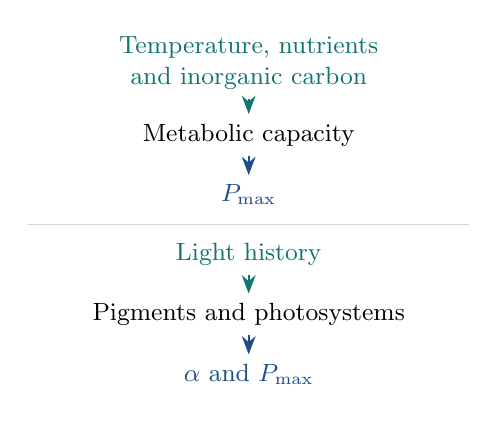
\begin{tikzpicture}[font=\small,>=Stealth,y=0.76cm]
 \node[text=accent,align=center] (temp) at (0,2.4) {Temperature, nutrients\\and inorganic carbon};
 \node[align=center] (met) at (0,1.2) {Metabolic capacity};
 \node[text=sea] (pmax) at (0,0.2) {$P_{\max}$};
 \draw[->,thick,accent] (temp)--(met);
 \draw[->,thick,sea] (met)--(pmax);
 \draw[grey!30] (-2.8,-0.3)--(2.8,-0.3);
 \node[text=accent] (light) at (0,-0.8) {Light history};
 \node[align=center] (pigment) at (0,-1.8) {Pigments and photosystems};
 \node[text=sea] (ap) at (0,-2.8) {$\alpha$ and $P_{\max}$};
 \draw[->,thick,accent] (light)--(pigment);
 \draw[->,thick,sea] (pigment)--(ap);
\end{tikzpicture}}
\vspace{0.5em}
\small $I_k$ changes when $P_{\max}/\alpha$ changes. $I_c$ also depends on respiration.
\fignote{A fall in $P_{\max}$ can indicate stress; check the species, light history and measurement conditions.}
\end{frame}

% 4: replaces BDC223_L06a_slide12.jpeg.
\begin{frame}{Light requirements differ among habitats}
\begin{columns}[c,onlytextwidth]
\begin{column}{0.55\textwidth}
\small
\textbf{Indicative values for seaweeds}\par
\vspace{0.5em}
$I_c$: about 2--11 in shallow water; it may be lower in deeper water.\par
\vspace{0.6em}
\renewcommand{\arraystretch}{1.5}
\begin{tabular}{@{}p{4.4cm}r@{}}
\toprule
\textbf{Habitat} & \textbf{$I_k$}\\
\midrule
Intertidal & 400--600\\
Upper to mid-sublittoral & 150--250\\
Deep water & $<100$\\
\bottomrule
\end{tabular}
\vspace{0.5em}
\par All irradiances in \lightunit.
\end{column}
\begin{column}{0.43\textwidth}
\centering
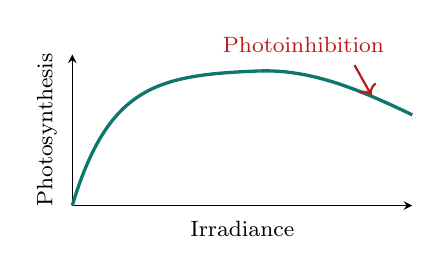
\begin{tikzpicture}
\begin{axis}[
 width=5.9cm,height=3.5cm,xmin=0,xmax=1,ymin=0,ymax=1,
 axis lines=left,xtick=\empty,ytick=\empty,xlabel={Irradiance},ylabel={Photosynthesis},
 label style={font=\footnotesize},clip=false]
 \addplot[accent,very thick,domain=0:0.55,samples=70] {0.9*(1-exp(-x/0.12))};
 \addplot[accent,very thick,domain=0.55:1,samples=60] {0.9*(1-exp(-x/0.12))*exp(-2*(x-0.55)^2)};
 \node[font=\footnotesize,text=rhodo,anchor=south,align=center] at (axis cs:0.68,0.95) {Photoinhibition};
 \draw[->,rhodo,thick] (axis cs:0.83,0.93)--(axis cs:0.88,0.73);
\end{axis}
\end{tikzpicture}
\small Excess light can reduce photosynthesis, especially when heat or drying adds stress.
\end{column}
\end{columns}
\vspace{0.6em}
\small Ice-diatom example: saturation near 5; photoinhibition near 25 (same units).
\fignote{Indicative examples from the original course notes, not universal thresholds. The curve is schematic.}
\end{frame}

% 5: replaces BDC223_L06a_slide13.jpeg.
\begin{frame}{Absorption spectra and action spectra}
\begin{columns}[t,onlytextwidth]
\begin{column}{0.47\textwidth}
\textcolor{accent}{\textbf{Absorption spectrum}}\par
\vspace{0.5em}
How much light is absorbed?\par
\vspace{0.8em}
\small At each wavelength, measure the light absorbed by pigments or tissue.\par
\vspace{0.5em}
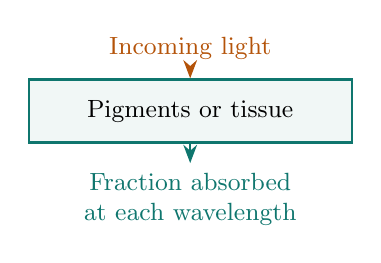
\begin{tikzpicture}[font=\small,>=Stealth,y=0.8cm]
 \node[text=warm] (in) at (0,1.6) {Incoming light};
 \node[draw=accent,thick,fill=accent!6,minimum width=4.1cm,minimum height=0.8cm] (sample) at (0,0.6) {Pigments or tissue};
 \node[align=center,text=accent] (out) at (0,-0.8) {Fraction absorbed\\at each wavelength};
 \draw[->,thick,warm] (in)--(sample);
 \draw[->,thick,accent] (sample)--(out);
\end{tikzpicture}
\end{column}
\begin{column}{0.47\textwidth}
\textcolor{sea}{\textbf{Action spectrum}}\par
\vspace{0.5em}
How much photosynthesis is driven?\par
\vspace{0.8em}
\small At each wavelength, measure a response such as oxygen production.\par
\vspace{0.5em}
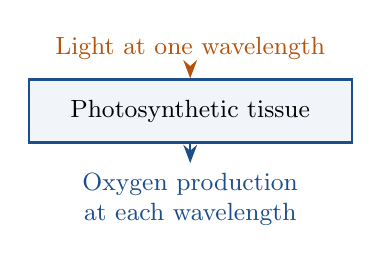
\begin{tikzpicture}[font=\small,>=Stealth,y=0.8cm]
 \node[text=warm] (in) at (0,1.6) {Light at one wavelength};
 \node[draw=sea,thick,fill=sea!6,minimum width=4.1cm,minimum height=0.8cm] (sample) at (0,0.6) {Photosynthetic tissue};
 \node[align=center,text=sea] (out) at (0,-0.8) {Oxygen production\\at each wavelength};
 \draw[->,thick,warm] (in)--(sample);
 \draw[->,thick,sea] (sample)--(out);
\end{tikzpicture}
\end{column}
\end{columns}
\vspace{0.5em}
\small\textcolor{warm}{Compare action at equal incident photon flux and at light levels below saturation.}
\fignote{Use matched tissue and conditions. Example: Haxo and Blinks (1950), marine algal action spectra.}
\end{frame}

% 6: replaces BDC223_L06a_slide14.jpeg.
\begin{frame}{Comparing absorption and action spectra}
\begin{columns}[c,onlytextwidth]
\begin{column}{0.63\textwidth}
\centering
\begin{tikzpicture}
\begin{axis}[
 width=8.4cm,height=4.8cm,xmin=400,xmax=700,ymin=0,ymax=1.1,
 domain=400:700,samples=201,axis lines=left,
 xlabel={Wavelength (nm)},ylabel={Relative value},
 xtick={400,450,500,550,600,650,700},ytick={0,0.5,1},
 tick label style={font=\footnotesize},label style={font=\small},
 grid=major,grid style={grey!13},
 legend style={font=\footnotesize,draw=none,fill=white,at={(0.5,1.04)},anchor=south,legend columns=1},
 legend cell align=left]
 \fill[warm!9] (axis cs:450,0) rectangle (axis cs:510,1.1);
 \addplot[accent,very thick] {(base(x)+0.58*band(x))/0.85};
 \addlegendentry{Absorption spectrum}
 \addplot[sea,very thick,dashed] {(base(x)+0.30*band(x))/0.85};
 \addlegendentry{Action spectrum (oxygen production)}
\end{axis}
\end{tikzpicture}
\end{column}
\begin{column}{0.35\textwidth}
\small
\begin{itemize}
 \item Similar peaks show where absorbed light drives photosynthesis
 \item In the shaded region, action is lower than absorption
 \item Some carotenoid excitation energy is dissipated before it reaches chlorophyll
\end{itemize}
\end{column}
\end{columns}
\vspace{0.3em}
\small Transfer efficiency differs among pigments and organisms; this pattern is an example.
\fignote{Schematic curves scaled to their maxima, not measurements. Related reading: Haxo and Blinks (1950).}
\end{frame}
\end{document}
